\documentclass[11pt]{article}
\usepackage{tikz}\usetikzlibrary{positioning}
\usepackage[margin=1in]{geometry}
\usepackage{fontspec}
\usepackage{longtable,array}
\usepackage{xcolor}
\definecolor{epgreen}{HTML}{428A5F}
\definecolor{epdarkgreen}{HTML}{214D35}
\usepackage[hidelinks]{hyperref}
\setlength{\parindent}{0pt}
\setlength{\parskip}{5pt}
\emergencystretch=3em
\sloppy
\title{Will Chicago Midway’s high land at 76–77°F?}
\author{\href{https://www.expectedparrot.com/}{\textcolor{epgreen}{\textbf{Expected Parrot}}}\\{\small Open-source research tools}\\[4pt]{\small Vorhersage | Forecast research report}}
\date{2026-09-16T15:20:34.447901Z}
\begin{document}
\maketitle
{\color{epgreen}\hrule height 1.5pt}\vspace{8pt}
\section*{\textcolor{epdarkgreen}{Assessment}}
Our sealed forecast is 24.4\%. Kalshi’s opening midpoint was 36.5\%, a 12.1-point disagreement. A predeclared 60-day reference class raised our initial estimate by 2.1 points but did not explain the market’s greater concentration in this narrow temperature band. The event remained unresolved at the forecast cutoff.


\section*{\textcolor{epdarkgreen}{The event and the forecast}}
Will Chicago Midway’s maximum temperature for September 17, 2026 be 76°F or 77°F? Our sealed estimate is 24.4\%, or roughly one chance in four. The Weather Company’s final CLIMDW report determines settlement for Kalshi contract KXHIGHCHI-26SEP17-B76.5. Midway is the relevant station; this is not an O’Hare forecast.


The event was still in the future when we sealed the estimate on September 16. A final daily maximum outside the two-degree band means No. Exceptional last-fair-price settlement or unavailable final data is outside this binary comparison. Forecast products and station observations are evidence, not the contractual settlement authority.


\clearpage
\section*{\textcolor{epdarkgreen}{Methodology at a glance}}
We saved the market quote first, then fixed the estimator before downloading historical outcomes. Evidence is shown in blue, assumptions in amber, and calculated results in green. The final quote comparison took place only after sealing the estimate.


\begin{center}
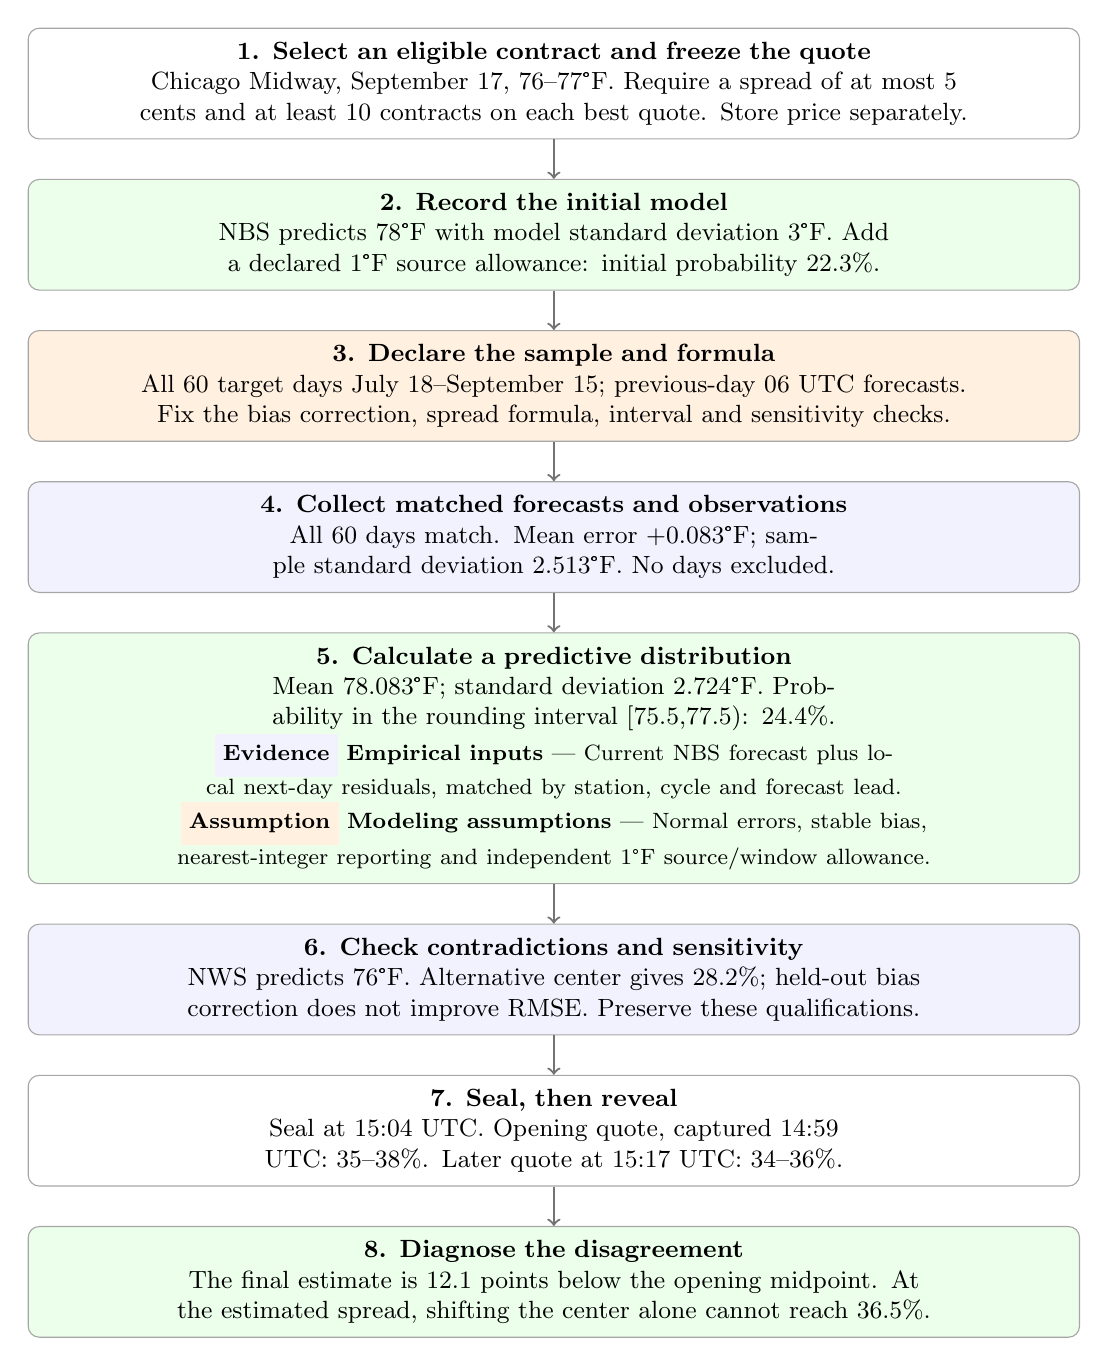
\begin{tikzpicture}[node distance=5mm, every node/.style={font=\small}]
\node[draw=black!35,rounded corners,align=center,text width=13cm,inner sep=5pt,fill=white] (flow0) {\textbf{1. Select an eligible contract and freeze the quote}\\ Chicago Midway, September 17, 76–77°F. Require a spread of at most 5 cents and at least 10 contracts on each best quote. Store price separately.};
\node[draw=black!35,rounded corners,align=center,text width=13cm,inner sep=5pt,fill=green!8,below=of flow0] (flow1) {\textbf{2. Record the initial model}\\ NBS predicts 78°F with model standard deviation 3°F. Add a declared 1°F source allowance: initial probability 22.3\%.};
\draw[->,thick,draw=black!55] (flow0.south) -- (flow1.north);
\node[draw=black!35,rounded corners,align=center,text width=13cm,inner sep=5pt,fill=orange!12,below=of flow1] (flow2) {\textbf{3. Declare the sample and formula}\\ All 60 target days July 18–September 15; previous-day 06 UTC forecasts. Fix the bias correction, spread formula, interval and sensitivity checks.};
\draw[->,thick,draw=black!55] (flow1.south) -- (flow2.north);
\node[draw=black!35,rounded corners,align=center,text width=13cm,inner sep=5pt,fill=blue!5,below=of flow2] (flow3) {\textbf{4. Collect matched forecasts and observations}\\ All 60 days match. Mean error +0.083°F; sample standard deviation 2.513°F. No days excluded.};
\draw[->,thick,draw=black!55] (flow2.south) -- (flow3.north);
\node[draw=black!35,rounded corners,align=center,text width=13cm,inner sep=5pt,fill=green!8,below=of flow3] (flow4) {\textbf{5. Calculate a predictive distribution}\\ Mean 78.083°F; standard deviation 2.724°F. Probability in the rounding interval [75.5,77.5): 24.4\%.\\{\footnotesize\colorbox{blue!5}{\strut\textbf{Evidence}} \textbf{Empirical inputs} — Current NBS forecast plus local next-day residuals, matched by station, cycle and forecast lead.}\\{\footnotesize\colorbox{orange!12}{\strut\textbf{Assumption}} \textbf{Modeling assumptions} — Normal errors, stable bias, nearest-integer reporting and independent 1°F source/window allowance.}};
\draw[->,thick,draw=black!55] (flow3.south) -- (flow4.north);
\node[draw=black!35,rounded corners,align=center,text width=13cm,inner sep=5pt,fill=blue!5,below=of flow4] (flow5) {\textbf{6. Check contradictions and sensitivity}\\ NWS predicts 76°F. Alternative center gives 28.2\%; held-out bias correction does not improve RMSE. Preserve these qualifications.};
\draw[->,thick,draw=black!55] (flow4.south) -- (flow5.north);
\node[draw=black!35,rounded corners,align=center,text width=13cm,inner sep=5pt,fill=white,below=of flow5] (flow6) {\textbf{7. Seal, then reveal}\\ Seal at 15:04 UTC. Opening quote, captured 14:59 UTC: 35–38\%. Later quote at 15:17 UTC: 34–36\%.};
\draw[->,thick,draw=black!55] (flow5.south) -- (flow6.north);
\node[draw=black!35,rounded corners,align=center,text width=13cm,inner sep=5pt,fill=green!8,below=of flow6] (flow7) {\textbf{8. Diagnose the disagreement}\\ The final estimate is 12.1 points below the opening midpoint. At the estimated spread, shifting the center alone cannot reach 36.5\%.};
\draw[->,thick,draw=black!55] (flow6.south) -- (flow7.north);
\end{tikzpicture}
\end{center}
{\small The executed sequence. Sample dates, forecast horizon, Gaussian estimator and extra uncertainty allowance were declared before collecting the historical sample.}
\clearpage
\section*{\textcolor{epdarkgreen}{How the prediction changed}}
Both probabilities were recorded before the opening quote was revealed. The smaller empirical error spread raised the probability of the narrow band; the estimated bias was close to zero. Kalshi was more confident that the high would land inside this particular band.


\begin{longtable}{>{\raggedright\arraybackslash}p{0.283\linewidth}>{\raggedright\arraybackslash}p{0.283\linewidth}>{\raggedright\arraybackslash}p{0.283\linewidth}}
\textbf{Stage} & \textbf{Probability} & \textbf{Gap below opening midpoint} \\ \hline\endhead
Initial NBS model & 22.3\% & 14.2 percentage points \\
After declared reference-class research & 24.4\% & 12.1 percentage points \\
Opening Kalshi midpoint & 36.5\% & Target, not an outcome \\
Later Kalshi midpoint & 35.0\% & Market movement reported separately \\
\end{longtable}
\section*{\textcolor{epdarkgreen}{Selection, timing and what was hidden}}
This is a one-question process-development exercise. We selected the next-day Chicago market to change both city and forecast horizon from the earlier NYC case. Selection was opportunistic, not a random sample of Kalshi contracts. The first bracket, 78–79°F, failed the ten-contract depth requirement. The adjacent 76–77°F bracket passed the same requirements; they were not relaxed.


The opening quote was captured at 14:59:25 UTC on September 16, before weather research. The initial probability and research plan were recorded at 15:01 UTC. The final checkpoint and seal were recorded at 15:04 UTC. The quote was revealed at 15:17:29 UTC. The initial forecast used the current NBS product, so it is not a completely uninformed prior.


The same assistant context handled the NYC and Chicago cases. The evaluator’s store was not inspected during research, but no separate context or enforced access barrier was used. No target probability was observed before sealing; contract thresholds were visible. Costs and model usage were not separately metered.


The opening order book had a 35-cent Yes bid and 38-cent Yes ask, with 24.02 and 20 contracts at those best quotes. About 92 bid-side and 101 ask-side contracts were within two cents of the best quotes. These figures establish that this snapshot passed the declared screen. They do not establish sustained depth, trading volume, or probability calibration.


\section*{\textcolor{epdarkgreen}{The reference class: matching the forecast we actually made}}
We paired every completed target day from July 18 through September 15 with its previous-day 06 UTC NBS forecast for KMDW. NOAA defines the daytime maximum TXN as covering 12 UTC through the following 06 UTC, reported at the following 00 UTC. For this next-day exercise, that is a 42-hour forecast lead. Matching the lead matters: same-day forecast errors would answer a different question.


IEM supplied both archived forecasts and MDW station daily maxima. All 60 dates were present; none were removed for unusually large errors. The average observation minus forecast was +0.083°F, with a sample standard deviation of 2.513°F. This sample shows almost no overall bias, but individual-day errors remain large compared with a two-degree contract band.


These are 60 consecutive late-summer days, not 60 independent weather experiments. Seasonal changes and persistent weather patterns limit transfer to tomorrow. IEM’s daily summaries and TWC’s final settlement values have not been shown to be identical. The live archive also does not certify exactly what data was available at each historical forecast time.


\par{\small Source: \href{https://mesonet.agron.iastate.edu/cgi-bin/request/mos.py?station=KMDW\&model=NBS\&sts=2026-07-17T00\%3A00Z\&ets=2026-09-15T00\%3A00Z\&format=csv}{IEM NBS forecast archive for Midway}}
\par{\small Source: \href{https://mesonet.agron.iastate.edu/cgi-bin/request/daily.py?sts=2026-07-18\&ets=2026-09-15\&network=IL\_ASOS\&stations=MDW\&var=max\_temp\_f\&format=csv}{IEM Midway station daily maxima}}
\par{\small Source: \href{https://mesonet.agron.iastate.edu/cgi-bin/request/daily.py?help=}{IEM daily-summary definitions}}
\par{\small Source: \href{https://vlab.noaa.gov/web/mdl/nbm-textcard-v5.0}{NOAA NBM station card definitions}}
\par{\small Source: \href{https://weather.com/kalshi}{The Weather Company climate data portal}}
\section*{\textcolor{epdarkgreen}{The calculation, including the subjective choices}}
The current 06 UTC NBS run predicts 78°F for September 17. Add the sample mean residual to obtain a predictive center of 78.083°F. Use residual variance multiplied by (1 + 1/60) to allow for uncertainty in the estimated mean, then add 1°F squared for a separately assumed source and reporting-window discrepancy. The resulting standard deviation is 2.724°F.


Assuming a normal distribution and nearest-integer reporting, a final report of 76°F or 77°F corresponds approximately to an underlying value from 75.5°F to 77.5°F. The area under this distribution over that interval is 24.3743\%. Decimal places make the computation reproducible; they do not indicate corresponding forecasting precision.


The model distribution, constant bias, 1°F allowance and rounding rule were all fixed before historical retrieval. They remain assumptions. The extra allowance is not estimated from a matched sample of TWC versus IEM reports. The simpler unsmoothed residual calculation puts 13 of 60 translated observations in the band, or 21.7\%.


\begin{longtable}{>{\raggedright\arraybackslash}p{0.283\linewidth}>{\raggedright\arraybackslash}p{0.283\linewidth}>{\raggedright\arraybackslash}p{0.283\linewidth}}
\textbf{Quantity} & \textbf{Value} & \textbf{Status} \\ \hline\endhead
Current NBS point forecast & 78°F & Observed forecast input \\
Historical mean residual & +0.083°F & Estimated from 60 proxy pairs \\
Historical residual spread & 2.513°F & Estimated sample standard deviation \\
Additional source/window spread & 1°F & Declared subjective assumption \\
Final distribution & Mean 78.083°F; SD 2.724°F & Gaussian model \\
Probability of 76–77°F & 24.4\% & Calculated under those assumptions \\
\end{longtable}
\par{\small Source: \href{https://mesonet.agron.iastate.edu/cgi-bin/request/mos.py?station=KMDW\&model=NBS\&sts=2026-07-17T00\%3A00Z\&ets=2026-09-15T00\%3A00Z\&format=csv}{IEM NBS forecast archive for Midway}}
\par{\small Source: \href{https://mesonet.agron.iastate.edu/cgi-bin/request/daily.py?sts=2026-07-18\&ets=2026-09-15\&network=IL\_ASOS\&stations=MDW\&var=max\_temp\_f\&format=csv}{IEM Midway station daily maxima}}
\par{\small Source: \href{https://vlab.noaa.gov/web/mdl/nbm-textcard-v5.0}{NOAA NBM station card definitions}}
\par{\small Source: \href{https://mesonet.agron.iastate.edu/cgi-bin/request/daily.py?help=}{IEM daily-summary definitions}}
\par{\small Source: \href{https://weather.com/kalshi}{The Weather Company climate data portal}}
\section*{\textcolor{epdarkgreen}{Checks that challenge the model}}
A chronological diagnostic fitted the first 40 days and checked the final 20. Uncorrected forecast RMSE was 2.559°F; applying the earlier sample’s bias made it slightly worse, at 2.596°F. Nineteen of the 20 observations fell within the model’s nominal 90\% interval. That is a small check, and does not demonstrate improved bias correction or reliable probability calibration. The final model still uses all 60 days because that choice was declared in advance.


The NWS Midway point forecast, updated at 10:45 UTC before the quote capture, predicts 76°F rather than NBS’s 78°F. The Chicago discussion describes showers and storms potentially lasting into Thursday morning, followed by drier conditions. Clouds, rain placement and wind direction create a plausible reason for forecast disagreement. We did not convert that narrative into an arbitrary numerical adjustment.


Using the NWS raw center of 76°F with the final model’s spread gives 28.2\%. We do not transfer the NBS bias correction to NWS, a different forecast product. Shifting our own final center by ±1°F yields 18.6–28.0\%; the full declared combination of mean shifts and 0–2°F extra spread yields 17.8–29.9\%. These are assumption sensitivities, not confidence intervals.


The TWC portal loaded, but its retrieved page shell and one inspected script did not provide an exact historical settlement series or establish rounding conventions. That check was limited. The report retains the provider mismatch rather than claiming the station archive resolved it.


\par{\small Source: \href{https://mesonet.agron.iastate.edu/cgi-bin/request/mos.py?station=KMDW\&model=NBS\&sts=2026-07-17T00\%3A00Z\&ets=2026-09-15T00\%3A00Z\&format=csv}{IEM NBS forecast archive for Midway}}
\par{\small Source: \href{https://mesonet.agron.iastate.edu/cgi-bin/request/daily.py?sts=2026-07-18\&ets=2026-09-15\&network=IL\_ASOS\&stations=MDW\&var=max\_temp\_f\&format=csv}{IEM Midway station daily maxima}}
\par{\small Source: \href{https://api.weather.gov/gridpoints/LOT/72,69/forecast}{NWS Midway point forecast}}
\par{\small Source: \href{https://forecast.weather.gov/product.php?site=LOT\&issuedby=LOT\&product=AFD\&format=TXT\&version=1\&glossary=0}{NWS Chicago forecast discussion}}
\par{\small Source: \href{https://mesonet.agron.iastate.edu/cgi-bin/request/daily.py?help=}{IEM daily-summary definitions}}
\par{\small Source: \href{https://vlab.noaa.gov/web/mdl/nbm-textcard-v5.0}{NOAA NBM station card definitions}}
\par{\small Source: \href{https://weather.com/kalshi}{The Weather Company climate data portal}}
\section*{\textcolor{epdarkgreen}{What comparison with Kalshi tells us}}
The opening midpoint was 36.5\%, making the final estimate 12.1 percentage points lower and 10.6 points below the opening bid. Research reduced squared distance from the opening midpoint from 0.02028 to 0.01470. This describes closer agreement on one selected case; it is not a Brier score and does not establish accuracy or a causal benefit from research.


The later quote was 34–36\%, midpoint 35\%, a decline of 1.5 points. The best later ask had only four contracts, below the ten-contract opening requirement. We preserve that later snapshot with this qualification and continue to use the opening target. The contract terms did not change.


A post-reveal diagnostic pinpoints a limitation: with standard deviation 2.724°F, the highest possible Gaussian probability in any two-degree interval is 28.65\%, achieved when centered exactly on that interval. Changing the point forecast alone therefore cannot reproduce the opening midpoint. An optimally centered Gaussian would require a standard deviation near 2.11°F to reach 36.5\%. That is a diagnosis of the disagreement, not a fitted replacement forecast or evidence that the market is right.


\section*{\textcolor{epdarkgreen}{The next process experiment}}
The main research opportunity is conditional uncertainty: does a model’s current dispersion, forecast lead and weather regime identify days with a narrower or wider error distribution? On a fresh hidden target, specify that conditioning method and a chronological validation procedure before inspecting outcomes. Use enough data to avoid carving a tiny, favorable reference class out of the history.


Also specify the latest available forecast cycle and obtain observations from the exact settlement source where possible. The 06 UTC run here was convenient for matching history, but was already several hours old when the target was captured. Retain this sealed 24.4\% forecast unchanged; evaluate the improved process on a new case.


\section*{\textcolor{epdarkgreen}{About this report}}
This explanation was written at report generation from the recorded research. It does not change the sealed predictions. The complete evidence and calculation records are in the technical appendix.


\clearpage
\appendix
\section{Technical appendix}
Complete records follow. These do not change the assessment above.
\subsection*{\textcolor{epdarkgreen}{Summary}}
Workbench workbench\_99\hspace{0pt}b666aae9114c\hspace{0pt}089f49: latest estimate 24.4\%; revealed.


\subsection*{\textcolor{epdarkgreen}{Question and resolution}}
\par\noindent\textbf{Created at:} 2026-09-16T14:59:21.853423Z

\par\noindent\textbf{Specification:} \par \par\noindent\textbf{Domain:} weather

\par\noindent\textbf{Event deadline:} 2026-09-18T06:00:00Z

\par\noindent\textbf{Event group:} KXHIGHCHI-26SEP17

\par\noindent\textbf{Id:} chicago\_high\_76\_77\_20260917

\par\noindent\textbf{Kind:} real

\par\noindent\textbf{No:} The final qualifying maximum is outside the inclusive 76–77°F bracket.

\par\noindent\textbf{Profile:} general

\par\noindent\textbf{Resolution source:} The Weather Company final CLIMDW daily maximum, per frozen Kalshi KXHIGHCHI rules and weather.com/kalshi. Forecasts and IEM station observations are research proxies.

\par\noindent\textbf{Resolve after:} 2026-09-19T06:00:00Z

\par\noindent\textbf{Text:} Will the maximum temperature reported for Chicago Midway (CLIMDW) on September 17, 2026 be 76–77°F?

\par\noindent\textbf{Void:} Last-fair-price settlement, unresolved material data errors, or unavailable final source data fall outside this binary comparison.

\par\noindent\textbf{Yes:} The Weather Company final maximum for Chicago CLIMDW for September 17, 2026 is in the inclusive 76–77°F bracket.

\par\noindent\textbf{Version:} 1

\subsection*{\textcolor{epdarkgreen}{Workbench overview}}
\par\noindent\textbf{Case id:} workbench\_99\hspace{0pt}b666aae9114c\hspace{0pt}089f49

\par\noindent\textbf{State:} revealed

\par\noindent\textbf{Question version:} 1

\par\noindent\textbf{Method:} Predeclared next-day weather residual model; hidden market comparison

\par\noindent\textbf{Mode:} prospective

\par\noindent\textbf{Latest estimate:} 24.4\%

\par\noindent\textbf{Sealed at:} 2026-09-16T15:04:10.490117Z

\par\noindent\textbf{Market status:} Revealed

\par\noindent\textbf{Opening target captured at:} 2026-09-16T14:59:25.889771Z

\subsection*{\textcolor{epdarkgreen}{Frozen contract and case selection}}
\par\noindent\textbf{Question:} \par \par\noindent\textbf{Created at:} 2026-09-16T14:59:21.853423Z

\par\noindent\textbf{Specification:} \par \par\noindent\textbf{Domain:} weather

\par\noindent\textbf{Event deadline:} 2026-09-18T06:00:00Z

\par\noindent\textbf{Event group:} KXHIGHCHI-26SEP17

\par\noindent\textbf{Id:} chicago\_high\_76\_77\_20260917

\par\noindent\textbf{Kind:} real

\par\noindent\textbf{No:} The final qualifying maximum is outside the inclusive 76–77°F bracket.

\par\noindent\textbf{Profile:} general

\par\noindent\textbf{Resolution source:} The Weather Company final CLIMDW daily maximum, per frozen Kalshi KXHIGHCHI rules and weather.com/kalshi. Forecasts and IEM station observations are research proxies.

\par\noindent\textbf{Resolve after:} 2026-09-19T06:00:00Z

\par\noindent\textbf{Text:} Will the maximum temperature reported for Chicago Midway (CLIMDW) on September 17, 2026 be 76–77°F?

\par\noindent\textbf{Void:} Last-fair-price settlement, unresolved material data errors, or unavailable final source data fall outside this binary comparison.

\par\noindent\textbf{Yes:} The Weather Company final maximum for Chicago CLIMDW for September 17, 2026 is in the inclusive 76–77°F bracket.

\par\noindent\textbf{Version:} 1

\par\noindent\textbf{Contract:} \par \par\noindent\textbf{Event group:} KXHIGHCHI-26SEP17

\par\noindent\textbf{Market id:} KXHIGHCHI-26SEP17-B76.5

\par\noindent\textbf{Resolution source:} See frozen Kalshi rules and series contract.

\par\noindent\textbf{Rules:} If the maximum temperature recorded at Chicago (CLIMDW) for Sep 17, 2026, is between 76-77° fahrenheit according to The Weather Company, then the market resolves to Yes.

Not all weather data is the same. While checking a source like AccuWeather or Google Weather may help guide your decision, the official and final value used to determine this market is the maximum/minimum temperature as reported by the Weather Company.

Reading weather data
Preliminary Weather Company data may be subject to rounding and conversion differences from the final reported value.
Use caution when interpreting preliminary Weather Company readings.

If it is determined in the sole discretion of the Exchange that there is a material error in the initial non-preliminary publication, Expiration may be held until the publication of a non-materially-erroneous data revision or until the Expiration Date, whichever comes first. If no data is available at the end of this period, all markets will resolve to the last fair price determined by Kalshi. Please note, a status of "Final" on weather.com/kalshi is provided for convenience only, and does not guarantee data to be error-free and thus exempt from the above.

\par\noindent\textbf{Scheduled close:} 2026-09-18T06:00:00Z

\par\noindent\textbf{Title:} Will the maximum temperature be 76-77° on Sep 17, 2026?

\par\noindent\textbf{Venue:} kalshi

\par\noindent\textbf{Yes description:} 76° to 77°

\par\noindent\textbf{Selection:} \par \par\noindent\textbf{Contract match rationale:} 76–77°F inclusive for CLIMDW, with TWC final reporting and error/last-fair-price exceptions. Daily date and trading close are recorded separately; cutoff uses end of local standard-time day.

\par\noindent\textbf{Eligibility rationale:} Tomorrow’s September 17 daily high is unobserved. The 78–79°F bracket failed the ten-contract depth requirement. This adjacent bracket is the second candidate, selected before weather research with the same thresholds.

\par\noindent\textbf{Market id:} KXHIGHCHI-26SEP17-B76.5

\par\noindent\textbf{Max spread:} 0.05

\par\noindent\textbf{Method:} Predeclared next-day weather residual model; hidden market comparison

\par\noindent\textbf{Min contracts each side:} 10

\par\noindent\textbf{Mode:} prospective

\par\noindent\textbf{Question:} \par \par\noindent\textbf{Question id:} chicago\_high\_76\_77\_20260917

\par\noindent\textbf{Version:} 1

\par\noindent\textbf{Venue:} kalshi

\subsection*{\textcolor{epdarkgreen}{Prediction history}}
Checkpoints are recorded judgments, not necessarily issued forecasts. All timestamps retain their recorded time zones.


\begin{longtable}{>{\raggedright\arraybackslash}p{.27\linewidth}>{\raggedright\arraybackslash}p{.65\linewidth}}
Stage & Initial \\
Probability & 22.3\% \\
Recorded at & 2026-09-16T15:01:06.843363Z \\
Gap to opening market (pp) & -14.24 \\
Squared market error & 0.020282 \\
Step improvement & Not applicable \\
\end{longtable}
\begin{longtable}{>{\raggedright\arraybackslash}p{.27\linewidth}>{\raggedright\arraybackslash}p{.65\linewidth}}
Stage & Research 1: How much do KMDW next-day NBS forecasts miss actual station daily maxima, and do current conditions make those residuals misleading? \\
Probability & 24.4\% \\
Recorded at & 2026-09-16T15:04:10.381702Z \\
Gap to opening market (pp) & -12.13 \\
Squared market error & 0.014703 \\
Step improvement & +0.005579 \\
\end{longtable}
\subsection*{\textcolor{epdarkgreen}{Market comparison}}
Frozen opening midpoint: 36.5\%; bid–ask 35.0\%–38.0\%. Captured 2026-09-16T14:59:25.889771Z.


Later midpoint: 35.0\%; bid–ask 34.0\%–36.0\%. Captured 2026-09-16T15:17:29.303904Z.


Squared market error = (estimate − opening midpoint)². Positive step improvement means closer agreement.


Market agreement is not an outcome score. The later quote is separate from the frozen opening target.


\par\noindent\textbf{Target:} \par \par\noindent\textbf{Ask:} 0.38

\par\noindent\textbf{Ask contracts within 2c:} 101.28999999999999

\par\noindent\textbf{Ask size:} 20.0

\par\noindent\textbf{Bid:} 0.35

\par\noindent\textbf{Bid contracts within 2c:} 92.02

\par\noindent\textbf{Bid size:} 24.02

\par\noindent\textbf{Midpoint:} 0.365

\par\noindent\textbf{Spread:} 0.03

\par\noindent\textbf{Target captured at:} 2026-09-16T14:59:25.889771Z

\par\noindent\textbf{Target method:} Opening order-book midpoint, frozen before initial assessment.

\par\noindent\textbf{Net squared error improvement:} 0.0055785531995272575

\par\noindent\textbf{Followup quote:} \par \par\noindent\textbf{Ask:} 0.36

\par\noindent\textbf{Ask contracts within 2c:} 52.6

\par\noindent\textbf{Ask size:} 4.0

\par\noindent\textbf{Bid:} 0.34

\par\noindent\textbf{Bid contracts within 2c:} 203.01

\par\noindent\textbf{Bid size:} 50.0

\par\noindent\textbf{Midpoint:} 0.35

\par\noindent\textbf{Spread:} 0.02

\par\noindent\textbf{Followup captured at:} 2026-09-16T15:17:29.303904Z

\par\noindent\textbf{Market movement pp:} -1.5000000000000013

\par\noindent\textbf{Followup error:} Not recorded

\par\noindent\textbf{Contract changed:} No

\par\noindent\textbf{Eligible for blind comparison:} Yes

\par\noindent\textbf{Qualification reasons:} \par None recorded.

\par\noindent\textbf{Limitations:} \par \par\noindent\textit{Item 1.}\par Market agreement is not an outcome score or proof of forecast accuracy.

\par\noindent\textit{Item 2.}\par Step improvements are descriptive; sequential research does not identify causal effects.

\par\noindent\textit{Item 3.}\par Research may include information arriving after the opening target. Inspect market movement and timestamps.

\par\noindent\textit{Item 4.}\par No exposure reported is an agent declaration, not independently verified isolation.

\par\noindent\textit{Item 5.}\par Bid-ask spread is not a confidence interval. Missing follow-up data does not replace the opening target.

\subsection*{\textcolor{epdarkgreen}{Research journal 1: Initial}}
Recorded 2026-09-16T15:01:06.843363Z · pre\_reveal


Entry workbench\_en\hspace{0pt}try\_4bbbd8eb\hspace{0pt}8a82494384a9


\par\noindent\textbf{Assumptions:} \par \par\noindent\textit{Item 1.}\par Gaussian error with zero bias initially

\par\noindent\textit{Item 2.}\par Model XND can serve as an initial spread proxy

\par\noindent\textit{Item 3.}\par Nearest-integer reporting approximation

\par\noindent\textit{Item 4.}\par Independent 1°F provider/window SD, selected before historical data

\par\noindent\textbf{Evidence refs:} \par \begin{longtable}{>{\raggedright\arraybackslash}p{0.440\linewidth}>{\raggedright\arraybackslash}p{0.440\linewidth}}
Packet id & Record id \\ \hline\endhead
pkt\_c687fdc6b2c6bac6de66623b & forecast78 \\
\end{longtable}

\par\noindent\textbf{Probability:} 22.3\%

\par\noindent\textbf{Rationale:} Frozen next-day NBS forecast is 78°F and model XND is 3°F. A declared Gaussian distribution with mean 78 and SD sqrt(3\textasciicircum{}2+1\textasciicircum{}2) incorporates a subjective independent 1°F settlement/provider allowance. Integrate over [75.5,77.5) for integer 76–77°F. This is model-based, not empirical calibration.

\par\noindent\textbf{Research status:} in\_progress

\par\noindent\textbf{Uncertainties:} \par \par\noindent\textit{Item 1.}\par Local next-day forecast bias and dispersion

\par\noindent\textit{Item 2.}\par TWC versus station reporting

\par\noindent\textit{Item 3.}\par Current synoptic conditions and alternative NWS forecast

\subsection*{\textcolor{epdarkgreen}{Research journal 2: Plan}}
Recorded 2026-09-16T15:01:06.951119Z · pre\_reveal


Entry workbench\_en\hspace{0pt}try\_af319ceb\hspace{0pt}bd5d4b228423


\par\noindent\textbf{Higher if:} Historical errors shift probability into 76–77°F or concentrate mass around that band; weather checks corroborate cooler conditions.

\par\noindent\textbf{Lower if:} Errors shift the center away from the band or increase dispersion; conditions show the next-day forecast is not a usable center.

\par\noindent\textbf{Search plan:} Primary estimator fixed now: include every target day July 18–September 15, 2026 (60 days). Pair IEM IL\_ASOS MDW daily max\_temp\_f with KMDW NBS previous-day 06 UTC TXN reported at target-day+1 00 UTC (42-hour lead). No outcome-based filtering; exclude only missing/non-numeric pairs and list them. Current center is fixed September 16 06 UTC TXN for September 17. Set mean = current TXN + sample mean residual (observed minus forecast); SD = sqrt(sample residual variance*(1+1/n)+1\textasciicircum{}2). Use Gaussian mass over [75.5,77.5). The 1°F provider/window SD and normality are declared assumptions. Do not choose a different estimator after observing market prices. Report unsmoothed empirical frequency and sensitivities to mean +/-1°F and extra SD 0,1,2°F. As a diagnostic only, fit bias and SD on first 40 complete chronological target days and report next 20 residual RMSE and interval coverage alongside unbiased raw forecasts. Minimum 30 valid pairs for revised estimator; otherwise retain initial and flag failure. Check TWC page for final-report conventions; check NOAA product definition, IEM daily definitions, current NWS point forecast and Chicago discussion. Preserve failed access and contradictions. NWS may motivate a labeled alternative-center sensitivity, not replace the fixed primary estimator.

\par\noindent\textbf{Stopping rule:} Stop after those defined sources and one complete 60-day extraction/calculation. No search for market odds. If definitions prevent a defensible mapping, report a qualified estimate or abort; do not silently change station, horizon, historical window, or liquidity requirements.

\par\noindent\textbf{Uncertainty:} How much do KMDW next-day NBS forecasts miss actual station daily maxima, and do current conditions make those residuals misleading?

\par\noindent\textbf{Why it matters:} This two-degree bracket is below the 78°F point forecast; small bias and spread changes can change its probability substantially.

\subsection*{\textcolor{epdarkgreen}{Research journal 3: Checkpoint}}
Recorded 2026-09-16T15:04:10.381702Z · pre\_reveal


Entry workbench\_en\hspace{0pt}try\_c5369e4c\hspace{0pt}e2114ee0b856 · Research plan workbench\_en\hspace{0pt}try\_af319ceb\hspace{0pt}bd5d4b228423


\par\noindent\textbf{Changed assumptions:} \par \par\noindent\textit{Item 1.}\par Empirical local next-day residual SD replaces model XND for primary spread.

\par\noindent\textit{Item 2.}\par Estimated mean residual+0.0833°F replaces initial zero-bias assumption.

\par\noindent\textit{Item 3.}\par Normality,1°F extra SD,and forecast product remain as declared before historical retrieval.

\par\noindent\textbf{Evidence refs:} \par \begin{longtable}{>{\raggedright\arraybackslash}p{0.440\linewidth}>{\raggedright\arraybackslash}p{0.440\linewidth}}
Packet id & Record id \\ \hline\endhead
pkt\_0f9495b8202397b68c559849 & residuals \\
pkt\_0f9495b8202397b68c559849 & holdout \\
pkt\_0f9495b8202397b68c559849 & weather\_disagreement \\
pkt\_0f9495b8202397b68c559849 & settlement\_gap \\
pkt\_0f9495b8202397b68c559849 & calculation \\
\end{longtable}

\par\noindent\textbf{Findings:} All60 matched days available. Bias+0.0833°F; residual SD2.5130°F. Holdout RMSE worsened slightly after bias correction. NWS76°F vs NBS78°F; cloudy/showery regime raises transfer uncertainty. TWC daily history and rounding remain unverified.

\par\noindent\textbf{Limitations:} \par \par\noindent\textit{Item 1.}\par IEM daily maxima are not exact TWC settlements.

\par\noindent\textit{Item 2.}\par NBS daytime maximum and full daily-report time windows differ.

\par\noindent\textit{Item 3.}\par Gaussian errors, constant bias, nearest-integer rounding and independent 1°F extra SD are assumptions.

\par\noindent\textit{Item 4.}\par 60 adjacent summer days may be correlated and may not match the current rainy autumn regime.

\par\noindent\textit{Item 5.}\par Forecast archive is retrieved now, not immutable original publication vintages.

\par\noindent\textit{Item 6.}\par Same assistant context as NYC; price separation is procedural, not enforced isolation.

\par\noindent\textit{Item 7.}\par Opening thresholds screen best quotes only, not trading volume or market calibration.

\par\noindent\textit{Item 8.}\par Usage and monetary costs are unmetered.

\par\noindent\textit{Item 9.}\par TWC portal check stopped at the public HTML and one script; no authenticated or comprehensive archive search was performed.

\par\noindent\textbf{Probability:} 24.4\%

\par\noindent\textbf{Rationale:} Apply the estimator fixed in the plan without changing its historical window, horizon, Gaussian assumption or 1°F extra spread. With mean78.0833°F and SD2.7240°F, the 76–77°F band has probability24.3743\%. Relative to the22.2586\% initial, lower estimated dispersion raises band mass; near-zero warm correction offsets a little. NWS disagrees on center, so report its28.19\% alternative without silently changing the declared model. The holdout does not support claiming the bias correction improves skill.

\par\noindent\textbf{Remaining uncertainties:} \par \par\noindent\textit{Item 1.}\par Whether summer pooled residuals transfer to tomorrow’s cloudy/rainy conditions

\par\noindent\textit{Item 2.}\par Which point forecast center is better for Midway

\par\noindent\textit{Item 3.}\par Exact TWC settlement versus IEM daily reporting

\par\noindent\textit{Item 4.}\par Serial dependence and small holdout sample

\par\noindent\textbf{Sources checked:} \par \par\noindent\textit{Item 1.}\par \href{https://mesonet.agron.iastate.edu/cgi-bin/request/mos.py?station=KMDW\&model=NBS\&sts=2026-07-17T00\%3A00Z\&ets=2026-09-15T00\%3A00Z\&format=csv}{https://meso\hspace{0pt}net.agron.ia\hspace{0pt}state.edu/cg\hspace{0pt}i-bin/reques\hspace{0pt}t/mos.py?sta\hspace{0pt}tion=KMDW\&mo\hspace{0pt}del=NBS\&sts=\hspace{0pt}2026-07-17T0\hspace{0pt}0\%3A00Z\&ets=\hspace{0pt}2026-09-15T0\hspace{0pt}0\%3A00Z\&form\hspace{0pt}at=csv}

\par\noindent\textit{Item 2.}\par \href{https://mesonet.agron.iastate.edu/cgi-bin/request/daily.py?sts=2026-07-18\&ets=2026-09-15\&network=IL\_ASOS\&stations=MDW\&var=max\_temp\_f\&format=csv}{https://meso\hspace{0pt}net.agron.ia\hspace{0pt}state.edu/cg\hspace{0pt}i-bin/reques\hspace{0pt}t/daily.py?s\hspace{0pt}ts=2026-07-1\hspace{0pt}8\&ets=2026-0\hspace{0pt}9-15\&network\hspace{0pt}=IL\_ASOS\&sta\hspace{0pt}tions=MDW\&va\hspace{0pt}r=max\_temp\_f\hspace{0pt}\&format=csv}

\par\noindent\textit{Item 3.}\par \href{https://api.weather.gov/gridpoints/LOT/72,69/forecast}{https://api.\hspace{0pt}weather.gov/\hspace{0pt}gridpoints/L\hspace{0pt}OT/72,69/for\hspace{0pt}ecast}

\par\noindent\textit{Item 4.}\par \href{https://forecast.weather.gov/product.php?site=LOT\&issuedby=LOT\&product=AFD\&format=TXT\&version=1\&glossary=0}{https://fore\hspace{0pt}cast.weather\hspace{0pt}.gov/product\hspace{0pt}.php?site=LO\hspace{0pt}T\&issuedby=L\hspace{0pt}OT\&product=A\hspace{0pt}FD\&format=TX\hspace{0pt}T\&version=1\&\hspace{0pt}glossary=0}

\par\noindent\textit{Item 5.}\par \href{https://mesonet.agron.iastate.edu/cgi-bin/request/daily.py?help=}{https://meso\hspace{0pt}net.agron.ia\hspace{0pt}state.edu/cg\hspace{0pt}i-bin/reques\hspace{0pt}t/daily.py?h\hspace{0pt}elp=}

\par\noindent\textit{Item 6.}\par \href{https://vlab.noaa.gov/web/mdl/nbm-textcard-v5.0}{https://vlab\hspace{0pt}.noaa.gov/we\hspace{0pt}b/mdl/nbm-te\hspace{0pt}xtcard-v5.0}

\par\noindent\textit{Item 7.}\par \href{https://weather.com/kalshi}{https://weather.com/kalshi}

\subsection*{\textcolor{epdarkgreen}{Research journal 4: Finish}}
Recorded 2026-09-16T15:04:10.490117Z · pre\_reveal


Entry workbench\_en\hspace{0pt}try\_c7aba215\hspace{0pt}be6b41879b2c


\par\noindent\textbf{Exposure notes:} No opening or outside probability for this event was seen or sought. Contract thresholds were visible. Same assistant context as NYC; evaluator storage was separate but accessible, with no enforced isolation. Market quote remains uninspected.

\par\noindent\textbf{Market exposure:} none

\par\noindent\textbf{Outcome status:} unresolved

\par\noindent\textbf{Stopping reason:} Completed the predeclared60-day extraction, chronological check, weather-source comparison and provider-definition checks. Remaining precision requires matched TWC settlement history or a separately validated regime model; do not tune further on this case.

\subsection*{\textcolor{epdarkgreen}{Research journal 5: Reflection}}
Recorded 2026-09-16T15:18:19.576095Z · post\_reveal


Entry workbench\_en\hspace{0pt}try\_f95519e1\hspace{0pt}d8a8418c8ce0


\par\noindent\textbf{Next method change:} On a new hidden-price case, predeclare a latest-available forecast cycle and a calibration method that conditions on forecast horizon and model dispersion or weather regime, using sufficiently many historical examples and a chronological holdout. Obtain exact settlement observations before fitting if possible. A centered Gaussian would need SD about2.11°F to match this opening midpoint; that is a post-reveal diagnostic, not permission to select that SD or rewrite this forecast. Treat the unresolved market as a development target, not proof of truth.

\par\noindent\textbf{What did not:} The final24.37\% remains below the35–38\% opening spread. With SD2.724°F, even a Gaussian centered optimally in the bracket has at most28.65\% probability, so merely substituting the cooler NWS center cannot close the gap. The later midpoint was35\% with only4 contracts at the best ask, failing our opening depth threshold. We lack exact TWC settlements and conditional forecast-error calibration.

\par\noindent\textbf{What helped:} Predeclaring the window, horizon and estimator made the calculation reproducible. All60 pairs were retained. Residual calibration reduced the opening-midpoint gap from14.24 to12.13 points; this is a descriptive change on one case. The chronological check surfaced that bias correction did not improve held-out RMSE.

\subsection*{\textcolor{epdarkgreen}{Model and calculation}}
No structured model artifact was attached to this case. The recorded rationales and assumptions above are the available model description. Supplemental files, if supplied, are identified separately below.


\subsection*{\textcolor{epdarkgreen}{Limitations and research cost}}
\par\noindent\textbf{Case limitations:} \par \par\noindent\textit{Item 1.}\par Prices are separated from this project, not protected by an operating-system sandbox.

\par\noindent\textit{Item 2.}\par Selection checks spread and top-of-book size only; neither establishes market accuracy.

\par\noindent\textit{Item 3.}\par The agent must verify the event is still unknown; an open market alone cannot establish this.

\par\noindent\textbf{Reported usage:} \par None recorded.

\par\noindent\textbf{Usage note:} Usage is agent-reported. Missing usage is unmetered, not zero; partial records are not a total.

\subsection*{\textcolor{epdarkgreen}{Supplemental model or research file: calculation.json}}
Supplied at report generation. This is not automatically part of the sealed research record; its hash can be compared with a previously recorded commitment. No code in this file was executed.


\par\noindent\textbf{Name:} calculation.json

\par\noindent\textbf{Sha256:} c9be200514ec\hspace{0pt}50e354c2149c\hspace{0pt}aa3e3a45cfd1\hspace{0pt}ac00a852fafa\hspace{0pt}3908ff01fd09\hspace{0pt}b7ae

\par\noindent\textbf{Provenance:} report\_time\_attachment

\par\noindent\textbf{Content:} \par \par\noindent\textbf{Selection:} All 60 target dates July 18–September 15, 2026; previous-day KMDW NBS 06 UTC; TXN at following-day 00 UTC (42-hour lead).

\par\noindent\textbf{Pairs:} \par \par\noindent\textit{Item 1.}\par \par\noindent\textbf{Date:} 2026-07-18

\par\noindent\textbf{Forecast:} 91.0

\par\noindent\textbf{Runtime:} 2026-07-17 06:00:00

\par\noindent\textbf{Forecast valid:} 2026-07-19 00:00:00

\par\noindent\textbf{Xnd:} 2.0

\par\noindent\textbf{Observed:} 91.0

\par\noindent\textbf{Error:} 0.0

\par\noindent\textit{Item 2.}\par \par\noindent\textbf{Date:} 2026-07-19

\par\noindent\textbf{Forecast:} 82.0

\par\noindent\textbf{Runtime:} 2026-07-18 06:00:00

\par\noindent\textbf{Forecast valid:} 2026-07-20 00:00:00

\par\noindent\textbf{Xnd:} 2.0

\par\noindent\textbf{Observed:} 79.0

\par\noindent\textbf{Error:} -3.0

\par\noindent\textit{Item 3.}\par \par\noindent\textbf{Date:} 2026-07-20

\par\noindent\textbf{Forecast:} 87.0

\par\noindent\textbf{Runtime:} 2026-07-19 06:00:00

\par\noindent\textbf{Forecast valid:} 2026-07-21 00:00:00

\par\noindent\textbf{Xnd:} 3.0

\par\noindent\textbf{Observed:} 82.0

\par\noindent\textbf{Error:} -5.0

\par\noindent\textit{Item 4.}\par \par\noindent\textbf{Date:} 2026-07-21

\par\noindent\textbf{Forecast:} 87.0

\par\noindent\textbf{Runtime:} 2026-07-20 06:00:00

\par\noindent\textbf{Forecast valid:} 2026-07-22 00:00:00

\par\noindent\textbf{Xnd:} 3.0

\par\noindent\textbf{Observed:} 86.0

\par\noindent\textbf{Error:} -1.0

\par\noindent\textit{Item 5.}\par \par\noindent\textbf{Date:} 2026-07-22

\par\noindent\textbf{Forecast:} 75.0

\par\noindent\textbf{Runtime:} 2026-07-21 06:00:00

\par\noindent\textbf{Forecast valid:} 2026-07-23 00:00:00

\par\noindent\textbf{Xnd:} 2.0

\par\noindent\textbf{Observed:} 73.0

\par\noindent\textbf{Error:} -2.0

\par\noindent\textit{Item 6.}\par \par\noindent\textbf{Date:} 2026-07-23

\par\noindent\textbf{Forecast:} 80.0

\par\noindent\textbf{Runtime:} 2026-07-22 06:00:00

\par\noindent\textbf{Forecast valid:} 2026-07-24 00:00:00

\par\noindent\textbf{Xnd:} 2.0

\par\noindent\textbf{Observed:} 77.0

\par\noindent\textbf{Error:} -3.0

\par\noindent\textit{Item 7.}\par \par\noindent\textbf{Date:} 2026-07-24

\par\noindent\textbf{Forecast:} 81.0

\par\noindent\textbf{Runtime:} 2026-07-23 06:00:00

\par\noindent\textbf{Forecast valid:} 2026-07-25 00:00:00

\par\noindent\textbf{Xnd:} 2.0

\par\noindent\textbf{Observed:} 79.0

\par\noindent\textbf{Error:} -2.0

\par\noindent\textit{Item 8.}\par \par\noindent\textbf{Date:} 2026-07-25

\par\noindent\textbf{Forecast:} 85.0

\par\noindent\textbf{Runtime:} 2026-07-24 06:00:00

\par\noindent\textbf{Forecast valid:} 2026-07-26 00:00:00

\par\noindent\textbf{Xnd:} 3.0

\par\noindent\textbf{Observed:} 79.0

\par\noindent\textbf{Error:} -6.0

\par\noindent\textit{Item 9.}\par \par\noindent\textbf{Date:} 2026-07-26

\par\noindent\textbf{Forecast:} 92.0

\par\noindent\textbf{Runtime:} 2026-07-25 06:00:00

\par\noindent\textbf{Forecast valid:} 2026-07-27 00:00:00

\par\noindent\textbf{Xnd:} 2.0

\par\noindent\textbf{Observed:} 91.0

\par\noindent\textbf{Error:} -1.0

\par\noindent\textit{Item 10.}\par \par\noindent\textbf{Date:} 2026-07-27

\par\noindent\textbf{Forecast:} 92.0

\par\noindent\textbf{Runtime:} 2026-07-26 06:00:00

\par\noindent\textbf{Forecast valid:} 2026-07-28 00:00:00

\par\noindent\textbf{Xnd:} 4.0

\par\noindent\textbf{Observed:} 88.0

\par\noindent\textbf{Error:} -4.0

\par\noindent\textit{Item 11.}\par \par\noindent\textbf{Date:} 2026-07-28

\par\noindent\textbf{Forecast:} 80.0

\par\noindent\textbf{Runtime:} 2026-07-27 06:00:00

\par\noindent\textbf{Forecast valid:} 2026-07-29 00:00:00

\par\noindent\textbf{Xnd:} 3.0

\par\noindent\textbf{Observed:} 79.0

\par\noindent\textbf{Error:} -1.0

\par\noindent\textit{Item 12.}\par \par\noindent\textbf{Date:} 2026-07-29

\par\noindent\textbf{Forecast:} 82.0

\par\noindent\textbf{Runtime:} 2026-07-28 06:00:00

\par\noindent\textbf{Forecast valid:} 2026-07-30 00:00:00

\par\noindent\textbf{Xnd:} 3.0

\par\noindent\textbf{Observed:} 80.0

\par\noindent\textbf{Error:} -2.0

\par\noindent\textit{Item 13.}\par \par\noindent\textbf{Date:} 2026-07-30

\par\noindent\textbf{Forecast:} 85.0

\par\noindent\textbf{Runtime:} 2026-07-29 06:00:00

\par\noindent\textbf{Forecast valid:} 2026-07-31 00:00:00

\par\noindent\textbf{Xnd:} 2.0

\par\noindent\textbf{Observed:} 86.0

\par\noindent\textbf{Error:} 1.0

\par\noindent\textit{Item 14.}\par \par\noindent\textbf{Date:} 2026-07-31

\par\noindent\textbf{Forecast:} 82.0

\par\noindent\textbf{Runtime:} 2026-07-30 06:00:00

\par\noindent\textbf{Forecast valid:} 2026-08-01 00:00:00

\par\noindent\textbf{Xnd:} 3.0

\par\noindent\textbf{Observed:} 82.0

\par\noindent\textbf{Error:} 0.0

\par\noindent\textit{Item 15.}\par \par\noindent\textbf{Date:} 2026-08-01

\par\noindent\textbf{Forecast:} 73.0

\par\noindent\textbf{Runtime:} 2026-07-31 06:00:00

\par\noindent\textbf{Forecast valid:} 2026-08-02 00:00:00

\par\noindent\textbf{Xnd:} 3.0

\par\noindent\textbf{Observed:} 76.0

\par\noindent\textbf{Error:} 3.0

\par\noindent\textit{Item 16.}\par \par\noindent\textbf{Date:} 2026-08-02

\par\noindent\textbf{Forecast:} 74.0

\par\noindent\textbf{Runtime:} 2026-08-01 06:00:00

\par\noindent\textbf{Forecast valid:} 2026-08-03 00:00:00

\par\noindent\textbf{Xnd:} 2.0

\par\noindent\textbf{Observed:} 76.0

\par\noindent\textbf{Error:} 2.0

\par\noindent\textit{Item 17.}\par \par\noindent\textbf{Date:} 2026-08-03

\par\noindent\textbf{Forecast:} 78.0

\par\noindent\textbf{Runtime:} 2026-08-02 06:00:00

\par\noindent\textbf{Forecast valid:} 2026-08-04 00:00:00

\par\noindent\textbf{Xnd:} 2.0

\par\noindent\textbf{Observed:} 82.0

\par\noindent\textbf{Error:} 4.0

\par\noindent\textit{Item 18.}\par \par\noindent\textbf{Date:} 2026-08-04

\par\noindent\textbf{Forecast:} 83.0

\par\noindent\textbf{Runtime:} 2026-08-03 06:00:00

\par\noindent\textbf{Forecast valid:} 2026-08-05 00:00:00

\par\noindent\textbf{Xnd:} 2.0

\par\noindent\textbf{Observed:} 86.0

\par\noindent\textbf{Error:} 3.0

\par\noindent\textit{Item 19.}\par \par\noindent\textbf{Date:} 2026-08-05

\par\noindent\textbf{Forecast:} 82.0

\par\noindent\textbf{Runtime:} 2026-08-04 06:00:00

\par\noindent\textbf{Forecast valid:} 2026-08-06 00:00:00

\par\noindent\textbf{Xnd:} 3.0

\par\noindent\textbf{Observed:} 83.0

\par\noindent\textbf{Error:} 1.0

\par\noindent\textit{Item 20.}\par \par\noindent\textbf{Date:} 2026-08-06

\par\noindent\textbf{Forecast:} 78.0

\par\noindent\textbf{Runtime:} 2026-08-05 06:00:00

\par\noindent\textbf{Forecast valid:} 2026-08-07 00:00:00

\par\noindent\textbf{Xnd:} 3.0

\par\noindent\textbf{Observed:} 80.0

\par\noindent\textbf{Error:} 2.0

\par\noindent\textit{Item 21.}\par \par\noindent\textbf{Date:} 2026-08-07

\par\noindent\textbf{Forecast:} 84.0

\par\noindent\textbf{Runtime:} 2026-08-06 06:00:00

\par\noindent\textbf{Forecast valid:} 2026-08-08 00:00:00

\par\noindent\textbf{Xnd:} 2.0

\par\noindent\textbf{Observed:} 86.0

\par\noindent\textbf{Error:} 2.0

\par\noindent\textit{Item 22.}\par \par\noindent\textbf{Date:} 2026-08-08

\par\noindent\textbf{Forecast:} 83.0

\par\noindent\textbf{Runtime:} 2026-08-07 06:00:00

\par\noindent\textbf{Forecast valid:} 2026-08-09 00:00:00

\par\noindent\textbf{Xnd:} 2.0

\par\noindent\textbf{Observed:} 84.0

\par\noindent\textbf{Error:} 1.0

\par\noindent\textit{Item 23.}\par \par\noindent\textbf{Date:} 2026-08-09

\par\noindent\textbf{Forecast:} 85.0

\par\noindent\textbf{Runtime:} 2026-08-08 06:00:00

\par\noindent\textbf{Forecast valid:} 2026-08-10 00:00:00

\par\noindent\textbf{Xnd:} 3.0

\par\noindent\textbf{Observed:} 86.0

\par\noindent\textbf{Error:} 1.0

\par\noindent\textit{Item 24.}\par \par\noindent\textbf{Date:} 2026-08-10

\par\noindent\textbf{Forecast:} 83.0

\par\noindent\textbf{Runtime:} 2026-08-09 06:00:00

\par\noindent\textbf{Forecast valid:} 2026-08-11 00:00:00

\par\noindent\textbf{Xnd:} 3.0

\par\noindent\textbf{Observed:} 88.0

\par\noindent\textbf{Error:} 5.0

\par\noindent\textit{Item 25.}\par \par\noindent\textbf{Date:} 2026-08-11

\par\noindent\textbf{Forecast:} 82.0

\par\noindent\textbf{Runtime:} 2026-08-10 06:00:00

\par\noindent\textbf{Forecast valid:} 2026-08-12 00:00:00

\par\noindent\textbf{Xnd:} 4.0

\par\noindent\textbf{Observed:} 80.0

\par\noindent\textbf{Error:} -2.0

\par\noindent\textit{Item 26.}\par \par\noindent\textbf{Date:} 2026-08-12

\par\noindent\textbf{Forecast:} 82.0

\par\noindent\textbf{Runtime:} 2026-08-11 06:00:00

\par\noindent\textbf{Forecast valid:} 2026-08-13 00:00:00

\par\noindent\textbf{Xnd:} 2.0

\par\noindent\textbf{Observed:} 83.0

\par\noindent\textbf{Error:} 1.0

\par\noindent\textit{Item 27.}\par \par\noindent\textbf{Date:} 2026-08-13

\par\noindent\textbf{Forecast:} 79.0

\par\noindent\textbf{Runtime:} 2026-08-12 06:00:00

\par\noindent\textbf{Forecast valid:} 2026-08-14 00:00:00

\par\noindent\textbf{Xnd:} 3.0

\par\noindent\textbf{Observed:} 77.0

\par\noindent\textbf{Error:} -2.0

\par\noindent\textit{Item 28.}\par \par\noindent\textbf{Date:} 2026-08-14

\par\noindent\textbf{Forecast:} 79.0

\par\noindent\textbf{Runtime:} 2026-08-13 06:00:00

\par\noindent\textbf{Forecast valid:} 2026-08-15 00:00:00

\par\noindent\textbf{Xnd:} 2.0

\par\noindent\textbf{Observed:} 80.0

\par\noindent\textbf{Error:} 1.0

\par\noindent\textit{Item 29.}\par \par\noindent\textbf{Date:} 2026-08-15

\par\noindent\textbf{Forecast:} 84.0

\par\noindent\textbf{Runtime:} 2026-08-14 06:00:00

\par\noindent\textbf{Forecast valid:} 2026-08-16 00:00:00

\par\noindent\textbf{Xnd:} 3.0

\par\noindent\textbf{Observed:} 81.0

\par\noindent\textbf{Error:} -3.0

\par\noindent\textit{Item 30.}\par \par\noindent\textbf{Date:} 2026-08-16

\par\noindent\textbf{Forecast:} 84.0

\par\noindent\textbf{Runtime:} 2026-08-15 06:00:00

\par\noindent\textbf{Forecast valid:} 2026-08-17 00:00:00

\par\noindent\textbf{Xnd:} 2.0

\par\noindent\textbf{Observed:} 86.0

\par\noindent\textbf{Error:} 2.0

\par\noindent\textit{Item 31.}\par \par\noindent\textbf{Date:} 2026-08-17

\par\noindent\textbf{Forecast:} 81.0

\par\noindent\textbf{Runtime:} 2026-08-16 06:00:00

\par\noindent\textbf{Forecast valid:} 2026-08-18 00:00:00

\par\noindent\textbf{Xnd:} 2.0

\par\noindent\textbf{Observed:} 78.0

\par\noindent\textbf{Error:} -3.0

\par\noindent\textit{Item 32.}\par \par\noindent\textbf{Date:} 2026-08-18

\par\noindent\textbf{Forecast:} 81.0

\par\noindent\textbf{Runtime:} 2026-08-17 06:00:00

\par\noindent\textbf{Forecast valid:} 2026-08-19 00:00:00

\par\noindent\textbf{Xnd:} 2.0

\par\noindent\textbf{Observed:} 81.0

\par\noindent\textbf{Error:} 0.0

\par\noindent\textit{Item 33.}\par \par\noindent\textbf{Date:} 2026-08-19

\par\noindent\textbf{Forecast:} 79.0

\par\noindent\textbf{Runtime:} 2026-08-18 06:00:00

\par\noindent\textbf{Forecast valid:} 2026-08-20 00:00:00

\par\noindent\textbf{Xnd:} 2.0

\par\noindent\textbf{Observed:} 80.0

\par\noindent\textbf{Error:} 1.0

\par\noindent\textit{Item 34.}\par \par\noindent\textbf{Date:} 2026-08-20

\par\noindent\textbf{Forecast:} 80.0

\par\noindent\textbf{Runtime:} 2026-08-19 06:00:00

\par\noindent\textbf{Forecast valid:} 2026-08-21 00:00:00

\par\noindent\textbf{Xnd:} 2.0

\par\noindent\textbf{Observed:} 78.0

\par\noindent\textbf{Error:} -2.0

\par\noindent\textit{Item 35.}\par \par\noindent\textbf{Date:} 2026-08-21

\par\noindent\textbf{Forecast:} 81.0

\par\noindent\textbf{Runtime:} 2026-08-20 06:00:00

\par\noindent\textbf{Forecast valid:} 2026-08-22 00:00:00

\par\noindent\textbf{Xnd:} 2.0

\par\noindent\textbf{Observed:} 80.0

\par\noindent\textbf{Error:} -1.0

\par\noindent\textit{Item 36.}\par \par\noindent\textbf{Date:} 2026-08-22

\par\noindent\textbf{Forecast:} 79.0

\par\noindent\textbf{Runtime:} 2026-08-21 06:00:00

\par\noindent\textbf{Forecast valid:} 2026-08-23 00:00:00

\par\noindent\textbf{Xnd:} 2.0

\par\noindent\textbf{Observed:} 82.0

\par\noindent\textbf{Error:} 3.0

\par\noindent\textit{Item 37.}\par \par\noindent\textbf{Date:} 2026-08-23

\par\noindent\textbf{Forecast:} 77.0

\par\noindent\textbf{Runtime:} 2026-08-22 06:00:00

\par\noindent\textbf{Forecast valid:} 2026-08-24 00:00:00

\par\noindent\textbf{Xnd:} 2.0

\par\noindent\textbf{Observed:} 76.0

\par\noindent\textbf{Error:} -1.0

\par\noindent\textit{Item 38.}\par \par\noindent\textbf{Date:} 2026-08-24

\par\noindent\textbf{Forecast:} 77.0

\par\noindent\textbf{Runtime:} 2026-08-23 06:00:00

\par\noindent\textbf{Forecast valid:} 2026-08-25 00:00:00

\par\noindent\textbf{Xnd:} 2.0

\par\noindent\textbf{Observed:} 79.0

\par\noindent\textbf{Error:} 2.0

\par\noindent\textit{Item 39.}\par \par\noindent\textbf{Date:} 2026-08-25

\par\noindent\textbf{Forecast:} 80.0

\par\noindent\textbf{Runtime:} 2026-08-24 06:00:00

\par\noindent\textbf{Forecast valid:} 2026-08-26 00:00:00

\par\noindent\textbf{Xnd:} 2.0

\par\noindent\textbf{Observed:} 81.0

\par\noindent\textbf{Error:} 1.0

\par\noindent\textit{Item 40.}\par \par\noindent\textbf{Date:} 2026-08-26

\par\noindent\textbf{Forecast:} 83.0

\par\noindent\textbf{Runtime:} 2026-08-25 06:00:00

\par\noindent\textbf{Forecast valid:} 2026-08-27 00:00:00

\par\noindent\textbf{Xnd:} 2.0

\par\noindent\textbf{Observed:} 85.0

\par\noindent\textbf{Error:} 2.0

\par\noindent\textit{Item 41.}\par \par\noindent\textbf{Date:} 2026-08-27

\par\noindent\textbf{Forecast:} 81.0

\par\noindent\textbf{Runtime:} 2026-08-26 06:00:00

\par\noindent\textbf{Forecast valid:} 2026-08-28 00:00:00

\par\noindent\textbf{Xnd:} 2.0

\par\noindent\textbf{Observed:} 81.0

\par\noindent\textbf{Error:} 0.0

\par\noindent\textit{Item 42.}\par \par\noindent\textbf{Date:} 2026-08-28

\par\noindent\textbf{Forecast:} 82.0

\par\noindent\textbf{Runtime:} 2026-08-27 06:00:00

\par\noindent\textbf{Forecast valid:} 2026-08-29 00:00:00

\par\noindent\textbf{Xnd:} 2.0

\par\noindent\textbf{Observed:} 84.0

\par\noindent\textbf{Error:} 2.0

\par\noindent\textit{Item 43.}\par \par\noindent\textbf{Date:} 2026-08-29

\par\noindent\textbf{Forecast:} 81.0

\par\noindent\textbf{Runtime:} 2026-08-28 06:00:00

\par\noindent\textbf{Forecast valid:} 2026-08-30 00:00:00

\par\noindent\textbf{Xnd:} 3.0

\par\noindent\textbf{Observed:} 82.0

\par\noindent\textbf{Error:} 1.0

\par\noindent\textit{Item 44.}\par \par\noindent\textbf{Date:} 2026-08-30

\par\noindent\textbf{Forecast:} 86.0

\par\noindent\textbf{Runtime:} 2026-08-29 06:00:00

\par\noindent\textbf{Forecast valid:} 2026-08-31 00:00:00

\par\noindent\textbf{Xnd:} 3.0

\par\noindent\textbf{Observed:} 81.0

\par\noindent\textbf{Error:} -5.0

\par\noindent\textit{Item 45.}\par \par\noindent\textbf{Date:} 2026-08-31

\par\noindent\textbf{Forecast:} 89.0

\par\noindent\textbf{Runtime:} 2026-08-30 06:00:00

\par\noindent\textbf{Forecast valid:} 2026-09-01 00:00:00

\par\noindent\textbf{Xnd:} 3.0

\par\noindent\textbf{Observed:} 91.0

\par\noindent\textbf{Error:} 2.0

\par\noindent\textit{Item 46.}\par \par\noindent\textbf{Date:} 2026-09-01

\par\noindent\textbf{Forecast:} 90.0

\par\noindent\textbf{Runtime:} 2026-08-31 06:00:00

\par\noindent\textbf{Forecast valid:} 2026-09-02 00:00:00

\par\noindent\textbf{Xnd:} 3.0

\par\noindent\textbf{Observed:} 94.0

\par\noindent\textbf{Error:} 4.0

\par\noindent\textit{Item 47.}\par \par\noindent\textbf{Date:} 2026-09-02

\par\noindent\textbf{Forecast:} 93.0

\par\noindent\textbf{Runtime:} 2026-09-01 06:00:00

\par\noindent\textbf{Forecast valid:} 2026-09-03 00:00:00

\par\noindent\textbf{Xnd:} 2.0

\par\noindent\textbf{Observed:} 96.0

\par\noindent\textbf{Error:} 3.0

\par\noindent\textit{Item 48.}\par \par\noindent\textbf{Date:} 2026-09-03

\par\noindent\textbf{Forecast:} 90.0

\par\noindent\textbf{Runtime:} 2026-09-02 06:00:00

\par\noindent\textbf{Forecast valid:} 2026-09-04 00:00:00

\par\noindent\textbf{Xnd:} 3.0

\par\noindent\textbf{Observed:} 92.0

\par\noindent\textbf{Error:} 2.0

\par\noindent\textit{Item 49.}\par \par\noindent\textbf{Date:} 2026-09-04

\par\noindent\textbf{Forecast:} 89.0

\par\noindent\textbf{Runtime:} 2026-09-03 06:00:00

\par\noindent\textbf{Forecast valid:} 2026-09-05 00:00:00

\par\noindent\textbf{Xnd:} 3.0

\par\noindent\textbf{Observed:} 93.0

\par\noindent\textbf{Error:} 4.0

\par\noindent\textit{Item 50.}\par \par\noindent\textbf{Date:} 2026-09-05

\par\noindent\textbf{Forecast:} 85.0

\par\noindent\textbf{Runtime:} 2026-09-04 06:00:00

\par\noindent\textbf{Forecast valid:} 2026-09-06 00:00:00

\par\noindent\textbf{Xnd:} 4.0

\par\noindent\textbf{Observed:} 83.0

\par\noindent\textbf{Error:} -2.0

\par\noindent\textit{Item 51.}\par \par\noindent\textbf{Date:} 2026-09-06

\par\noindent\textbf{Forecast:} 77.0

\par\noindent\textbf{Runtime:} 2026-09-05 06:00:00

\par\noindent\textbf{Forecast valid:} 2026-09-07 00:00:00

\par\noindent\textbf{Xnd:} 2.0

\par\noindent\textbf{Observed:} 79.0

\par\noindent\textbf{Error:} 2.0

\par\noindent\textit{Item 52.}\par \par\noindent\textbf{Date:} 2026-09-07

\par\noindent\textbf{Forecast:} 79.0

\par\noindent\textbf{Runtime:} 2026-09-06 06:00:00

\par\noindent\textbf{Forecast valid:} 2026-09-08 00:00:00

\par\noindent\textbf{Xnd:} 2.0

\par\noindent\textbf{Observed:} 80.0

\par\noindent\textbf{Error:} 1.0

\par\noindent\textit{Item 53.}\par \par\noindent\textbf{Date:} 2026-09-08

\par\noindent\textbf{Forecast:} 87.0

\par\noindent\textbf{Runtime:} 2026-09-07 06:00:00

\par\noindent\textbf{Forecast valid:} 2026-09-09 00:00:00

\par\noindent\textbf{Xnd:} 2.0

\par\noindent\textbf{Observed:} 87.0

\par\noindent\textbf{Error:} 0.0

\par\noindent\textit{Item 54.}\par \par\noindent\textbf{Date:} 2026-09-09

\par\noindent\textbf{Forecast:} 83.0

\par\noindent\textbf{Runtime:} 2026-09-08 06:00:00

\par\noindent\textbf{Forecast valid:} 2026-09-10 00:00:00

\par\noindent\textbf{Xnd:} 3.0

\par\noindent\textbf{Observed:} 80.0

\par\noindent\textbf{Error:} -3.0

\par\noindent\textit{Item 55.}\par \par\noindent\textbf{Date:} 2026-09-10

\par\noindent\textbf{Forecast:} 78.0

\par\noindent\textbf{Runtime:} 2026-09-09 06:00:00

\par\noindent\textbf{Forecast valid:} 2026-09-11 00:00:00

\par\noindent\textbf{Xnd:} 2.0

\par\noindent\textbf{Observed:} 76.0

\par\noindent\textbf{Error:} -2.0

\par\noindent\textit{Item 56.}\par \par\noindent\textbf{Date:} 2026-09-11

\par\noindent\textbf{Forecast:} 79.0

\par\noindent\textbf{Runtime:} 2026-09-10 06:00:00

\par\noindent\textbf{Forecast valid:} 2026-09-12 00:00:00

\par\noindent\textbf{Xnd:} 2.0

\par\noindent\textbf{Observed:} 81.0

\par\noindent\textbf{Error:} 2.0

\par\noindent\textit{Item 57.}\par \par\noindent\textbf{Date:} 2026-09-12

\par\noindent\textbf{Forecast:} 85.0

\par\noindent\textbf{Runtime:} 2026-09-11 06:00:00

\par\noindent\textbf{Forecast valid:} 2026-09-13 00:00:00

\par\noindent\textbf{Xnd:} 2.0

\par\noindent\textbf{Observed:} 88.0

\par\noindent\textbf{Error:} 3.0

\par\noindent\textit{Item 58.}\par \par\noindent\textbf{Date:} 2026-09-13

\par\noindent\textbf{Forecast:} 75.0

\par\noindent\textbf{Runtime:} 2026-09-12 06:00:00

\par\noindent\textbf{Forecast valid:} 2026-09-14 00:00:00

\par\noindent\textbf{Xnd:} 3.0

\par\noindent\textbf{Observed:} 75.0

\par\noindent\textbf{Error:} 0.0

\par\noindent\textit{Item 59.}\par \par\noindent\textbf{Date:} 2026-09-14

\par\noindent\textbf{Forecast:} 75.0

\par\noindent\textbf{Runtime:} 2026-09-13 06:00:00

\par\noindent\textbf{Forecast valid:} 2026-09-15 00:00:00

\par\noindent\textbf{Xnd:} 3.0

\par\noindent\textbf{Observed:} 71.0

\par\noindent\textbf{Error:} -4.0

\par\noindent\textit{Item 60.}\par \par\noindent\textbf{Date:} 2026-09-15

\par\noindent\textbf{Forecast:} 84.0

\par\noindent\textbf{Runtime:} 2026-09-14 06:00:00

\par\noindent\textbf{Forecast valid:} 2026-09-16 00:00:00

\par\noindent\textbf{Xnd:} 4.0

\par\noindent\textbf{Observed:} 85.0

\par\noindent\textbf{Error:} 1.0

\par\noindent\textbf{Excluded dates:} \par None recorded.

\par\noindent\textbf{N:} 60

\par\noindent\textbf{Current nbs high f:} 78.0

\par\noindent\textbf{Current nbs xnd f:} 3.0

\par\noindent\textbf{Initial probability:} 0.22258588036127136

\par\noindent\textbf{Bias observed minus forecast f:} 0.08333333333333333

\par\noindent\textbf{Residual sample sd f:} 2.5129607540533594

\par\noindent\textbf{Final mean f:} 78.08333333333333

\par\noindent\textbf{Final sd f:} 2.724008311404838

\par\noindent\textbf{Assumed extra provider window sd f:} 1

\par\noindent\textbf{Final probability:} 0.243743131027777

\par\noindent\textbf{Empirical residual probability:} 0.21666666666666667

\par\noindent\textbf{Holdout diagnostic:} \par \par\noindent\textbf{Train n:} 40

\par\noindent\textbf{Test n:} 20

\par\noindent\textbf{Train bias f:} -0.15

\par\noindent\textbf{Train sd f:} 2.4863731180277995

\par\noindent\textbf{Raw rmse f:} 2.5592967784139455

\par\noindent\textbf{Bias corrected rmse f:} 2.595669470483482

\par\noindent\textbf{Nominal 90pct interval coverage:} 0.95

\par\noindent\textbf{Interval halfwidth f:} 4.45527743722064

\par\noindent\textbf{Qualification:} One small chronological check on proxy observations; not validation against TWC settlements.

\par\noindent\textbf{Nws alternative:} \par \par\noindent\textbf{High f:} 76

\par\noindent\textbf{Issued at:} 2026-09-16T10:45:49+00:00

\par\noindent\textbf{Probability with nws center and same sd:} 0.28188425711116283

\par\noindent\textbf{Qualification:} Alternative raw NWS center; NBS bias is not transferred to a different forecast product. This is sensitivity, not the selected forecast.

\par\noindent\textbf{Sensitivity:} \par \begin{longtable}{>{\raggedright\arraybackslash}p{0.293\linewidth}>{\raggedright\arraybackslash}p{0.293\linewidth}>{\raggedright\arraybackslash}p{0.293\linewidth}}
Extra sd f & Mean shift f & Probability \\ \hline\endhead
0 & -1 & 0.2992839849741104 \\
0 & 0 & 0.2549879895849905 \\
0 & 1 & 0.18737362900274696 \\
1 & -1 & 0.2802498776230036 \\
1 & 0 & 0.243743131027777 \\
1 & 1 & 0.18635845463066886 \\
2 & -1 & 0.23945969355425462 \\
2 & 0 & 0.2165239485849555 \\
2 & 1 & 0.17840678562263984 \\
\end{longtable}

\par\noindent\textbf{Limitations:} \par \par\noindent\textit{Item 1.}\par IEM daily maxima are not exact TWC settlements.

\par\noindent\textit{Item 2.}\par NBS daytime maximum and full daily-report time windows differ.

\par\noindent\textit{Item 3.}\par Gaussian errors, constant bias, nearest-integer rounding and independent 1°F extra SD are assumptions.

\par\noindent\textit{Item 4.}\par 60 adjacent summer days may be correlated and may not match the current rainy autumn regime.

\par\noindent\textit{Item 5.}\par Forecast archive is retrieved now, not immutable original publication vintages.

\par\noindent\textit{Item 6.}\par Same assistant context as NYC; price separation is procedural, not enforced isolation.

\par\noindent\textit{Item 7.}\par Opening thresholds screen best quotes only, not trading volume or market calibration.

\par\noindent\textbf{Raw sha256:} \par \par\noindent\textbf{Daily definitions.html:} 618a63cf7860\hspace{0pt}efde3a662086\hspace{0pt}4351d293e3de\hspace{0pt}c75dfb0729fa\hspace{0pt}b344c20c22d3\hspace{0pt}57b9

\par\noindent\textbf{Nbm definitions.html:} 5115c4313054\hspace{0pt}bce18faa03b4\hspace{0pt}9b98b7f38512\hspace{0pt}ed35e56dacf0\hspace{0pt}319006286bcb\hspace{0pt}0079

\par\noindent\textbf{Nbs current.json:} 7ba9e336d42d\hspace{0pt}64a8fd049bdf\hspace{0pt}4574bd399c07\hspace{0pt}c16f779d2075\hspace{0pt}1697a831ad30\hspace{0pt}f141

\par\noindent\textbf{Nbs history.csv:} 71ac8307e2f7\hspace{0pt}e098fcd7f787\hspace{0pt}5f920af7d590\hspace{0pt}83352f68e209\hspace{0pt}4dc9319cf8bb\hspace{0pt}8c70

\par\noindent\textbf{Nws discussion.html:} 89ba7c14d8ac\hspace{0pt}7ee72f001ceb\hspace{0pt}278807398308\hspace{0pt}52f04242aa67\hspace{0pt}f045cceee9b5\hspace{0pt}6e9d

\par\noindent\textbf{Nws forecast.json:} 9e71052ea0bf\hspace{0pt}5a780777597d\hspace{0pt}f45ecf29eab7\hspace{0pt}2c83cbed3a6d\hspace{0pt}91b0d90d00c4\hspace{0pt}f24d

\par\noindent\textbf{Nws points.json:} b75739325a7d\hspace{0pt}1daff7eb9aeb\hspace{0pt}d6a7c9d50fa7\hspace{0pt}832b5cddc146\hspace{0pt}8f7889496ae4\hspace{0pt}4b8a

\par\noindent\textbf{Observed history.csv:} 67f8ea837fad\hspace{0pt}85346b0b4d62\hspace{0pt}da6a945bc61e\hspace{0pt}b7a98a7540c3\hspace{0pt}8b81abd5e62a\hspace{0pt}1eb5

\par\noindent\textbf{Twc.html:} 8687c886fda4\hspace{0pt}87d41824a695\hspace{0pt}86c280d7aebd\hspace{0pt}7e2988f4db33\hspace{0pt}d608b1490f8f\hspace{0pt}ee8b

\subsection*{\textcolor{epdarkgreen}{Finding: pkt\_c687fdc6\hspace{0pt}b2c6bac6de66\hspace{0pt}623b:forecas\hspace{0pt}t78}}
Sources: [1], [2]


\par\noindent\textbf{Claim:} At the next-day horizon the frozen NBS forecast is 78°F with a 3°F reported model standard deviation. XND is model uncertainty, not independently demonstrated error calibration.

\par\noindent\textbf{Claim type:} observation

\par\noindent\textbf{Entity ids:} \par None recorded.

\par\noindent\textbf{Id:} forecast78

\par\noindent\textbf{Observed at:} 2026-09-16T1\hspace{0pt}5:00:28.3365\hspace{0pt}55+00:00

\par\noindent\textbf{Provenance:} \par \par\noindent\textbf{Adapter:} vorhersage.r\hspace{0pt}esearch\_bund\hspace{0pt}le.v1

\par\noindent\textbf{Value:} Not recorded

\subsection*{\textcolor{epdarkgreen}{Finding: pkt\_0f9495b8\hspace{0pt}202397b68c55\hspace{0pt}9849:residua\hspace{0pt}ls}}
Sources: [3], [4]


\par\noindent\textbf{Claim:} All 60 predefined days were matched without exclusions. Mean observed-minus-NBS error is 0.083333°F; sample SD is 2.512961°F.

\par\noindent\textbf{Claim type:} inference

\par\noindent\textbf{Entity ids:} \par None recorded.

\par\noindent\textbf{Id:} residuals

\par\noindent\textbf{Observed at:} 2026-09-16T1\hspace{0pt}5:01:23.3579\hspace{0pt}79+00:00

\par\noindent\textbf{Provenance:} \par \par\noindent\textbf{Adapter:} vorhersage.r\hspace{0pt}esearch\_bund\hspace{0pt}le.v1

\par\noindent\textbf{Value:} Not recorded

\subsection*{\textcolor{epdarkgreen}{Finding: pkt\_0f9495b8\hspace{0pt}202397b68c55\hspace{0pt}9849:holdout}}
Sources: [3], [4]


\par\noindent\textbf{Claim:} Fitting on the first 40 days and checking the last 20: raw forecast RMSE 2.5593°F, bias-corrected RMSE 2.5957°F; 19/20 observations lie in the declared nominal 90\% interval. This small check does not demonstrate improved bias correction or calibration.

\par\noindent\textbf{Claim type:} inference

\par\noindent\textbf{Entity ids:} \par None recorded.

\par\noindent\textbf{Id:} holdout

\par\noindent\textbf{Observed at:} 2026-09-16T1\hspace{0pt}5:01:23.3579\hspace{0pt}79+00:00

\par\noindent\textbf{Provenance:} \par \par\noindent\textbf{Adapter:} vorhersage.r\hspace{0pt}esearch\_bund\hspace{0pt}le.v1

\par\noindent\textbf{Value:} Not recorded

\subsection*{\textcolor{epdarkgreen}{Finding: pkt\_0f9495b8\hspace{0pt}202397b68c55\hspace{0pt}9849:weather\hspace{0pt}\_disagreemen\hspace{0pt}t}}
Sources: [5], [6]


\par\noindent\textbf{Claim:} NWS Thursday point forecast is 76°F versus NBS 78°F; rain timing, cloud cover and wind direction remain uncertain. With the same final spread, using the raw NWS center gives 28.19\%. This is an alternative assumption, not an independent probability vote.

\par\noindent\textbf{Claim type:} inference

\par\noindent\textbf{Entity ids:} \par None recorded.

\par\noindent\textbf{Id:} weather\_disagreement

\par\noindent\textbf{Observed at:} 2026-09-16T1\hspace{0pt}5:01:20.8879\hspace{0pt}29+00:00

\par\noindent\textbf{Provenance:} \par \par\noindent\textbf{Adapter:} vorhersage.r\hspace{0pt}esearch\_bund\hspace{0pt}le.v1

\par\noindent\textbf{Value:} Not recorded

\subsection*{\textcolor{epdarkgreen}{Finding: pkt\_0f9495b8\hspace{0pt}202397b68c55\hspace{0pt}9849:settlem\hspace{0pt}ent\_gap}}
Sources: [7], [8], [9]


\par\noindent\textbf{Claim:} No matched TWC settlement history or exact rounding convention was extracted. Station and NBS windows differ; the 1°F extra spread is an explicit assumption, not an empirically measured settlement correction.

\par\noindent\textbf{Claim type:} inference

\par\noindent\textbf{Entity ids:} \par None recorded.

\par\noindent\textbf{Id:} settlement\_gap

\par\noindent\textbf{Observed at:} 2026-09-16T1\hspace{0pt}5:01:21.1394\hspace{0pt}91+00:00

\par\noindent\textbf{Provenance:} \par \par\noindent\textbf{Adapter:} vorhersage.r\hspace{0pt}esearch\_bund\hspace{0pt}le.v1

\par\noindent\textbf{Value:} Not recorded

\subsection*{\textcolor{epdarkgreen}{Finding: pkt\_0f9495b8\hspace{0pt}202397b68c55\hspace{0pt}9849:calcula\hspace{0pt}tion}}
Sources: [3], [4], [8]


\par\noindent\textbf{Claim:} The predeclared estimator gives mean 78.083333°F, SD 2.724008°F and probability 0.243743131. Empirical unsmoothed estimate is 13/60=21.67\%. Mean shifts +/-1°F give 18.64–28.02\%. Calculation SHA256: c9be200514ec\hspace{0pt}50e354c2149c\hspace{0pt}aa3e3a45cfd1\hspace{0pt}ac00a852fafa\hspace{0pt}3908ff01fd09\hspace{0pt}b7ae

\par\noindent\textbf{Claim type:} inference

\par\noindent\textbf{Entity ids:} \par None recorded.

\par\noindent\textbf{Id:} calculation

\par\noindent\textbf{Observed at:} 2026-09-16T1\hspace{0pt}5:01:23.3579\hspace{0pt}79+00:00

\par\noindent\textbf{Provenance:} \par \par\noindent\textbf{Adapter:} vorhersage.r\hspace{0pt}esearch\_bund\hspace{0pt}le.v1

\par\noindent\textbf{Value:} Not recorded

\subsection*{\textcolor{epdarkgreen}{Source [1]: IEM archived NBS 06 UTC forecast for Midway}}
\par\noindent\textbf{Excerpt:} September 16 06 UTC run gives September 17 daytime maximum TXN 78°F and XND 3°F, reported at September 18 00 UTC.

\par\noindent\textbf{Excerpt kind:} paraphrase

\par\noindent\textbf{Id:} current

\par\noindent\textbf{Retrieved at:} 2026-09-16T1\hspace{0pt}5:00:28.3365\hspace{0pt}55+00:00

\par\noindent\textbf{Title:} IEM archived NBS 06 UTC forecast for Midway

\par\noindent\textbf{Url:} \href{https://mesonet.agron.iastate.edu/api/1/mos.json?station=KMDW\&model=NBS\&runtime=2026-09-16T06\%3A00Z}{https://meso\hspace{0pt}net.agron.ia\hspace{0pt}state.edu/ap\hspace{0pt}i/1/mos.json\hspace{0pt}?station=KMD\hspace{0pt}W\&model=NBS\&\hspace{0pt}runtime=2026\hspace{0pt}-09-16T06\%3A\hspace{0pt}00Z}

\subsection*{\textcolor{epdarkgreen}{Source [2]: NOAA NBM station card definitions}}
\par\noindent\textbf{Excerpt:} NBS maximum TXN spans 12 UTC through following-day 06 UTC and is reported at following-day 00 UTC. XND is the maximum/minimum temperature standard deviation in Fahrenheit.

\par\noindent\textbf{Excerpt kind:} paraphrase

\par\noindent\textbf{Id:} definitions

\par\noindent\textbf{Retrieved at:} 2026-09-16T1\hspace{0pt}5:00:28.3365\hspace{0pt}55+00:00

\par\noindent\textbf{Title:} NOAA NBM station card definitions

\par\noindent\textbf{Url:} \href{https://vlab.noaa.gov/web/mdl/nbm-textcard-v5.0}{https://vlab\hspace{0pt}.noaa.gov/we\hspace{0pt}b/mdl/nbm-te\hspace{0pt}xtcard-v5.0}

\subsection*{\textcolor{epdarkgreen}{Source [3]: IEM NBS forecast archive for Midway}}
\par\noindent\textbf{Excerpt:} All 60 target dates have a previous-day 06 UTC KMDW NBS forecast with 42-hour TXN. Forecast dates run July 17 through September 14.

\par\noindent\textbf{Excerpt kind:} paraphrase

\par\noindent\textbf{Id:} history

\par\noindent\textbf{Retrieved at:} 2026-09-16T1\hspace{0pt}5:01:23.3579\hspace{0pt}79+00:00

\par\noindent\textbf{Title:} IEM NBS forecast archive for Midway

\par\noindent\textbf{Url:} \href{https://mesonet.agron.iastate.edu/cgi-bin/request/mos.py?station=KMDW\&model=NBS\&sts=2026-07-17T00\%3A00Z\&ets=2026-09-15T00\%3A00Z\&format=csv}{https://meso\hspace{0pt}net.agron.ia\hspace{0pt}state.edu/cg\hspace{0pt}i-bin/reques\hspace{0pt}t/mos.py?sta\hspace{0pt}tion=KMDW\&mo\hspace{0pt}del=NBS\&sts=\hspace{0pt}2026-07-17T0\hspace{0pt}0\%3A00Z\&ets=\hspace{0pt}2026-09-15T0\hspace{0pt}0\%3A00Z\&form\hspace{0pt}at=csv}

\subsection*{\textcolor{epdarkgreen}{Source [4]: IEM Midway station daily maxima}}
\par\noindent\textbf{Excerpt:} All 60 predetermined target dates July 18 through September 15 have a station daily high. These are proxy observations, not verified TWC settlements.

\par\noindent\textbf{Excerpt kind:} paraphrase

\par\noindent\textbf{Id:} observed

\par\noindent\textbf{Retrieved at:} 2026-09-16T1\hspace{0pt}5:01:20.7661\hspace{0pt}25+00:00

\par\noindent\textbf{Title:} IEM Midway station daily maxima

\par\noindent\textbf{Url:} \href{https://mesonet.agron.iastate.edu/cgi-bin/request/daily.py?sts=2026-07-18\&ets=2026-09-15\&network=IL\_ASOS\&stations=MDW\&var=max\_temp\_f\&format=csv}{https://meso\hspace{0pt}net.agron.ia\hspace{0pt}state.edu/cg\hspace{0pt}i-bin/reques\hspace{0pt}t/daily.py?s\hspace{0pt}ts=2026-07-1\hspace{0pt}8\&ets=2026-0\hspace{0pt}9-15\&network\hspace{0pt}=IL\_ASOS\&sta\hspace{0pt}tions=MDW\&va\hspace{0pt}r=max\_temp\_f\hspace{0pt}\&format=csv}

\subsection*{\textcolor{epdarkgreen}{Source [5]: NWS Midway point forecast}}
\par\noindent\textbf{Excerpt:} NWS forecasts September 17 high near 76°F, mostly cloudy, with possible showers and thunderstorms before 1pm. This is 2°F below the frozen NBS point forecast.

\par\noindent\textbf{Excerpt kind:} paraphrase

\par\noindent\textbf{Id:} nws

\par\noindent\textbf{Published at:} 2026-09-16T10:45:49Z

\par\noindent\textbf{Retrieved at:} 2026-09-16T1\hspace{0pt}5:01:20.5835\hspace{0pt}47+00:00

\par\noindent\textbf{Title:} NWS Midway point forecast

\par\noindent\textbf{Url:} \href{https://api.weather.gov/gridpoints/LOT/72,69/forecast}{https://api.\hspace{0pt}weather.gov/\hspace{0pt}gridpoints/L\hspace{0pt}OT/72,69/for\hspace{0pt}ecast}

\subsection*{\textcolor{epdarkgreen}{Source [6]: NWS Chicago forecast discussion}}
\par\noindent\textbf{Excerpt:} Rain and storms may affect Thursday morning; drier conditions are expected later. The location of heavier overnight rain is uncertain. Clouds, wind direction and precipitation create regime uncertainty in daily highs.

\par\noindent\textbf{Excerpt kind:} paraphrase

\par\noindent\textbf{Id:} discussion

\par\noindent\textbf{Published at:} 2026-09-16T12:00:00Z

\par\noindent\textbf{Retrieved at:} 2026-09-16T1\hspace{0pt}5:01:20.8879\hspace{0pt}29+00:00

\par\noindent\textbf{Title:} NWS Chicago forecast discussion

\par\noindent\textbf{Url:} \href{https://forecast.weather.gov/product.php?site=LOT\&issuedby=LOT\&product=AFD\&format=TXT\&version=1\&glossary=0}{https://fore\hspace{0pt}cast.weather\hspace{0pt}.gov/product\hspace{0pt}.php?site=LO\hspace{0pt}T\&issuedby=L\hspace{0pt}OT\&product=A\hspace{0pt}FD\&format=TX\hspace{0pt}T\&version=1\&\hspace{0pt}glossary=0}

\subsection*{\textcolor{epdarkgreen}{Source [7]: IEM daily-summary definitions}}
\par\noindent\textbf{Excerpt:} The archive mixes computed calendar-day summaries and explicit official totals. Airport daily windows typically follow standard time, or 1am to 1am daylight time.

\par\noindent\textbf{Excerpt kind:} paraphrase

\par\noindent\textbf{Id:} daily\_definition

\par\noindent\textbf{Retrieved at:} 2026-09-16T1\hspace{0pt}5:01:21.1394\hspace{0pt}91+00:00

\par\noindent\textbf{Title:} IEM daily-summary definitions

\par\noindent\textbf{Url:} \href{https://mesonet.agron.iastate.edu/cgi-bin/request/daily.py?help=}{https://meso\hspace{0pt}net.agron.ia\hspace{0pt}state.edu/cg\hspace{0pt}i-bin/reques\hspace{0pt}t/daily.py?h\hspace{0pt}elp=}

\subsection*{\textcolor{epdarkgreen}{Source [8]: NOAA NBM station card definitions}}
\par\noindent\textbf{Excerpt:} NBS maximum TXN spans 12 UTC through next-day 06 UTC and appears at next-day 00 UTC. XND measures model maximum/minimum temperature standard deviation.

\par\noindent\textbf{Excerpt kind:} paraphrase

\par\noindent\textbf{Id:} nbm\_definition

\par\noindent\textbf{Retrieved at:} 2026-09-16T1\hspace{0pt}4:59:41.5932\hspace{0pt}73+00:00

\par\noindent\textbf{Title:} NOAA NBM station card definitions

\par\noindent\textbf{Url:} \href{https://vlab.noaa.gov/web/mdl/nbm-textcard-v5.0}{https://vlab\hspace{0pt}.noaa.gov/we\hspace{0pt}b/mdl/nbm-te\hspace{0pt}xtcard-v5.0}

\subsection*{\textcolor{epdarkgreen}{Source [9]: The Weather Company climate data portal}}
\par\noindent\textbf{Excerpt:} The public HTML presents a climate portal with daily and hourly views. The retrieved shell and one script did not establish a historical TWC settlement series, exact rounding, or full daily-window conventions.

\par\noindent\textbf{Excerpt kind:} paraphrase

\par\noindent\textbf{Id:} twc

\par\noindent\textbf{Retrieved at:} 2026-09-16T1\hspace{0pt}5:01:20.6498\hspace{0pt}53+00:00

\par\noindent\textbf{Title:} The Weather Company climate data portal

\par\noindent\textbf{Url:} \href{https://weather.com/kalshi}{https://weather.com/kalshi}

\subsection*{\textcolor{epdarkgreen}{Report provenance}}
This report renders stored records without new research, model calls, or probability revisions. Missing work remains missing. The JSON export preserves the complete report input.


\par\noindent\textbf{Schema version:} vorhersage.report.v1

\par\noindent\textbf{Generated at:} 2026-09-16T15:20:34.447901Z

\par\noindent\textbf{Record sha256:} 7d5815bd1c54\hspace{0pt}0e5f1b8c296b\hspace{0pt}1905028a7710\hspace{0pt}190563285610\hspace{0pt}fd19b8d39356\hspace{0pt}123f

\par\noindent\textbf{Format:} latex

\par\noindent\textbf{Latex engine:} XeLaTeX or LuaLaTeX

\par\noindent\textbf{Narrative sha256:} 2b4a1f2755a1\hspace{0pt}e08684db331f\hspace{0pt}4bfb89510e3e\hspace{0pt}4618c63f4d1d\hspace{0pt}965f127c4c1c\hspace{0pt}5e9d

\end{document}
